\documentclass{article}

\usepackage{amsmath}
\usepackage{float}

\usepackage{graphicx}
\graphicspath{ {../outputs/} }

\usepackage[style=numeric, backend=bibtex8]{biblatex}
\addbibresource{citations.bib}

\begin{document}

  \title{Linear Time Generation of Simulated Wireless Sensor Networks with Random Geometric Graphs}
  \author{Luke Wood}
  \maketitle

  \section{Executive Summary}
  \subsection{Introduction and Summary}
	Wireless Sensor Networks can be incredibly expensive to deploy and test which makes them an excellent candidate for simulated testing.
	Vlady Ravelomananana and Hichem Kenniche from the University of Paris first explored the concept of using random geometric graphs (RGGs) to attempt to model wireless sensor networks \cite{kenniche2010random}.
	RGGs can be used as a relatively cheap way to gather valuable information about how wireless sensor networks can function and communicate.
	Through a series of reports	I will be:
	\begin{enumerate}
		\item Generating RGGs on the geometries of a unit square, unit disc, and unit sphere
		\item Color the generated graph in linear time using smallest vertex last ordering (TODO check)
		\item Find the terminal clique in the generated RGGs
		\item Find a selection of bipartite subgraphs producted by an algorithm for coloring
	\end{enumerate}
	This report is the first of the series and  will describe an implementation for a linear time algorithm to generate graphs consisting of N vertices with an average degree of A on the geometric topologies of: unit square, unit disc, unit sphere.

	\begin{center}
	  \begin{table}[H]
			\begin{tabular}{ |c|c|c|c|c|c| }
				\hline
				Nodes & Expected Avg. Deg. & Real Avg. Deg. & Max Deg. & Min Deg. & Seconds \\
        \hline
        1000 & 64 & 57.568000 & 82 & 10 & 0.279913 \\
        \hline
        5000 & 64 & 60.658400 & 87 & 15 & 0.840636 \\
        \hline
        25000 & 64 & 62.504080 & 98 & 11 & 3.828407 \\
        \hline
        50000 & 64 & 62.986840 & 100 & 20 & 8.938070 \\
        \hline
        100000 & 64 & 63.258520 & 102 & 18 & 14.938207 \\
        \hline

			\end{tabular}
			\caption{Data on graphs generated with the square topology}
		\end{table}
	\end{center}

  Currently, my implementation has support for:
  \begin{enumerate}
    \item Generating a unit square topology RGG
    \item Converting that RGG to an Adjacency List
    \item Serializing Adjacency Lists to files
  \end{enumerate}
  Being able to serialize the Adjacency Lists to files is a noteworthy feature as if there are algorithms that require faster runtimes than a dynamically typed language can support (such as python) we can still generate the RGGs from my implementation and use them elsewhere.

  \subsection{Programming Environment Description}
  	The implementation of the algorithm used to gather the data supporting this report was gathered on a 15 inch Macbook pro 2017 with a 2.9 GHz Intel Core i7 processor and 16 GB of RAM.
    The computer is running macOS High Sierra.
    The graph generation is written in python 3 as generating and connection a graph is not super computationally expensive with even decently large inputs such as 100000.
    The later algorithms may be implemented in a different language such as Elixir to get high levels of concurrency and higher efficiency due to type inference (as opposed to pythons dynamic typing
    )
  \section{Reduction to Practice}
	  \subsection{Data Structure Design}
    In the generation portion of this project I use
	  \subsection{Algorithm Description}
    In order to ensure that average degree of the nodes is close to the desired average degree we define a radius surrounding each node.
    The formulas to find the radius for each topology is derived from the equations found in the paper Bipartite Grid Partitioning of a Random Geometric Graph\cite{chen2017bipartite}.
    The formula used to find this radius varies for each graph tolopogy and can be found in the table displayed below:

    \begin{tabular}{ |c|c|c| }
  	  \hline
  	  Topology & Equation in Chen's Paper & Equation for Radius Derive from Chen's \\
  	  \hline
  	  Unit Square & $d(G) \approx N\pi r^2 $ & $r = sqrt(\dfrac{d(G)}{N\pi})$ \\
  	  \hline
  	  Unit Disc   & & \\
  	  \hline
  	  Unit Sphere & & \\
  	  \hline
    \end{tabular}

	  \subsection{Algorithm Engineering}
	  Originally I had a brute force algorithm that ran in $O(n^2)$ time.
	  This quickly became problematic as the algorithm took upwards of 200 seconds to run on input size of only 12,000.
	  \begin{figure}[H]
		\centering
		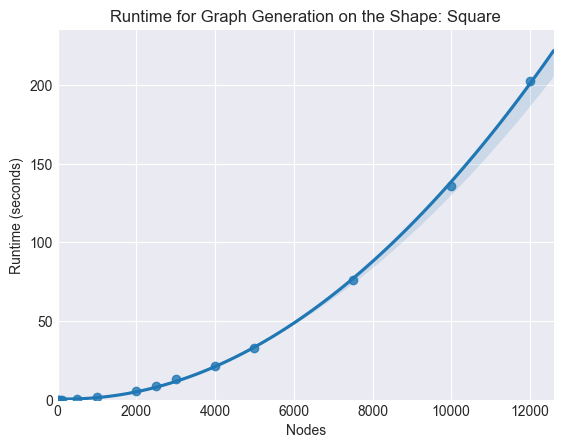
\includegraphics[width=1 \textwidth]{square/runtime/runtime_chart_naive}
		\caption{Runtimes of the $O(n^2)$ Algorithm}
	  \end{figure}


	  To fix this, I overhauled the algorithm to be $O(n)$.
	  I did this by implementing the cell method described above in the Algorithm Description section as well as in Chen's paper Bipartite Grid Partitioning of a Random Geometric Graph\cite{chen2017bipartite}.
	  \begin{figure}[H]
		\centering
		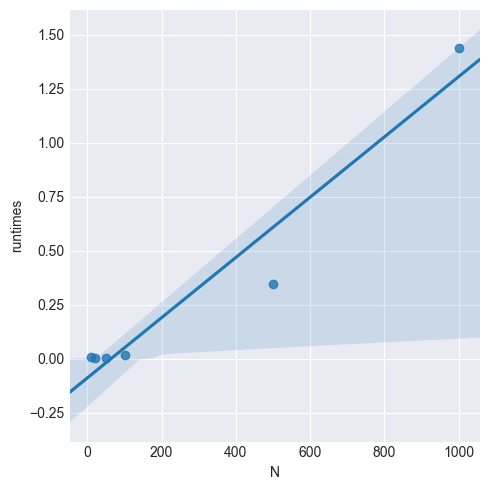
\includegraphics[width=1 \textwidth]{square/runtime/runtime_chart}
		\caption{Runtimes of the $O(n)$ Algorithm}
	  \end{figure}

	  I have also included a table to compare some of the runtimes for the same size inputs below.

	  \begin{center}
	  \begin{table}[H]
		\begin{tabular}{ |c|c|c| }
			\hline
			Nodes & $O(n^2)$ & $O(n)$ \\
			\hline
      1000 & 0.258400 & 0.657174 \\
      \hline
      2000 & 0.382116 & 2.630040 \\
      \hline
      3000 & 0.473916 & 5.874501 \\
      \hline
      5000 & 0.831753 & 16.809004 \\
      \hline
      10000 & 1.560216 & 65.398991 \\
			\hline
		\end{tabular}
		\caption{Runtimes of the $O(n)$ and $O(n^2)$ algorithms in seconds}
	  \end{table}
	  \end{center}

	  The $O(n)$ algorithm is far superior even on small input sizes such as 1000.

	\subsection{Verification}

\section{Result Summary}
  \subsection{Edge Density}
  As expected I got a gaussian distribution for my edge densities.
  \begin{figure}[H]
  \centering
  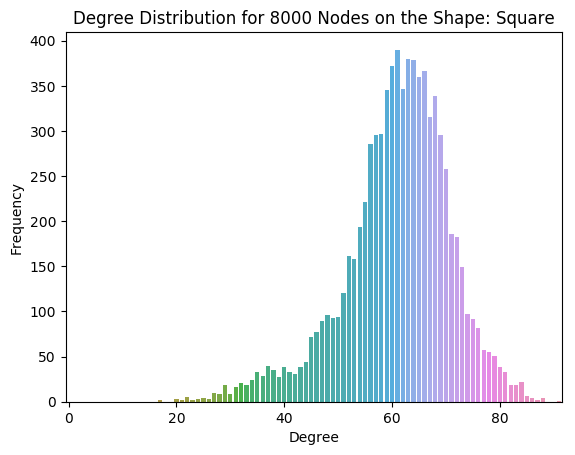
\includegraphics[width=1 \textwidth]{square/edge_density/8000_64.png}
  \caption{Edge Densities of an 8000 Node Graph with E(Degree)=64}
  \end{figure}

  \subsection{Performance Rates}
  \begin{center}
	  \begin{table}[H]
		  \begin{tabular}{ |c|c|c| }
			\hline
			Nodes & Topology & Runtime \\
			\hline
		  \end{tabular}
		  \caption{Runtimes of the $O(n)$ vertex connection algorithm}
	  \end{table}
  \end{center}

\printbibliography

\end{document}
